% Options for packages loaded elsewhere
\PassOptionsToPackage{unicode}{hyperref}
\PassOptionsToPackage{hyphens}{url}
%
\documentclass[
]{article}
\usepackage{lmodern}
\usepackage{amssymb,amsmath}
\usepackage{ifxetex,ifluatex}
\ifnum 0\ifxetex 1\fi\ifluatex 1\fi=0 % if pdftex
  \usepackage[T1]{fontenc}
  \usepackage[utf8]{inputenc}
  \usepackage{textcomp} % provide euro and other symbols
\else % if luatex or xetex
  \usepackage{unicode-math}
  \defaultfontfeatures{Scale=MatchLowercase}
  \defaultfontfeatures[\rmfamily]{Ligatures=TeX,Scale=1}
\fi
% Use upquote if available, for straight quotes in verbatim environments
\IfFileExists{upquote.sty}{\usepackage{upquote}}{}
\IfFileExists{microtype.sty}{% use microtype if available
  \usepackage[]{microtype}
  \UseMicrotypeSet[protrusion]{basicmath} % disable protrusion for tt fonts
}{}
\makeatletter
\@ifundefined{KOMAClassName}{% if non-KOMA class
  \IfFileExists{parskip.sty}{%
    \usepackage{parskip}
  }{% else
    \setlength{\parindent}{0pt}
    \setlength{\parskip}{6pt plus 2pt minus 1pt}}
}{% if KOMA class
  \KOMAoptions{parskip=half}}
\makeatother
\usepackage{xcolor}
\IfFileExists{xurl.sty}{\usepackage{xurl}}{} % add URL line breaks if available
\IfFileExists{bookmark.sty}{\usepackage{bookmark}}{\usepackage{hyperref}}
\hypersetup{
  pdftitle={1. Regresja liniowa},
  pdfauthor={Michał Maj},
  hidelinks,
  pdfcreator={LaTeX via pandoc}}
\urlstyle{same} % disable monospaced font for URLs
\usepackage[margin=1in]{geometry}
\usepackage{color}
\usepackage{fancyvrb}
\newcommand{\VerbBar}{|}
\newcommand{\VERB}{\Verb[commandchars=\\\{\}]}
\DefineVerbatimEnvironment{Highlighting}{Verbatim}{commandchars=\\\{\}}
% Add ',fontsize=\small' for more characters per line
\usepackage{framed}
\definecolor{shadecolor}{RGB}{248,248,248}
\newenvironment{Shaded}{\begin{snugshade}}{\end{snugshade}}
\newcommand{\AlertTok}[1]{\textcolor[rgb]{0.94,0.16,0.16}{#1}}
\newcommand{\AnnotationTok}[1]{\textcolor[rgb]{0.56,0.35,0.01}{\textbf{\textit{#1}}}}
\newcommand{\AttributeTok}[1]{\textcolor[rgb]{0.77,0.63,0.00}{#1}}
\newcommand{\BaseNTok}[1]{\textcolor[rgb]{0.00,0.00,0.81}{#1}}
\newcommand{\BuiltInTok}[1]{#1}
\newcommand{\CharTok}[1]{\textcolor[rgb]{0.31,0.60,0.02}{#1}}
\newcommand{\CommentTok}[1]{\textcolor[rgb]{0.56,0.35,0.01}{\textit{#1}}}
\newcommand{\CommentVarTok}[1]{\textcolor[rgb]{0.56,0.35,0.01}{\textbf{\textit{#1}}}}
\newcommand{\ConstantTok}[1]{\textcolor[rgb]{0.00,0.00,0.00}{#1}}
\newcommand{\ControlFlowTok}[1]{\textcolor[rgb]{0.13,0.29,0.53}{\textbf{#1}}}
\newcommand{\DataTypeTok}[1]{\textcolor[rgb]{0.13,0.29,0.53}{#1}}
\newcommand{\DecValTok}[1]{\textcolor[rgb]{0.00,0.00,0.81}{#1}}
\newcommand{\DocumentationTok}[1]{\textcolor[rgb]{0.56,0.35,0.01}{\textbf{\textit{#1}}}}
\newcommand{\ErrorTok}[1]{\textcolor[rgb]{0.64,0.00,0.00}{\textbf{#1}}}
\newcommand{\ExtensionTok}[1]{#1}
\newcommand{\FloatTok}[1]{\textcolor[rgb]{0.00,0.00,0.81}{#1}}
\newcommand{\FunctionTok}[1]{\textcolor[rgb]{0.00,0.00,0.00}{#1}}
\newcommand{\ImportTok}[1]{#1}
\newcommand{\InformationTok}[1]{\textcolor[rgb]{0.56,0.35,0.01}{\textbf{\textit{#1}}}}
\newcommand{\KeywordTok}[1]{\textcolor[rgb]{0.13,0.29,0.53}{\textbf{#1}}}
\newcommand{\NormalTok}[1]{#1}
\newcommand{\OperatorTok}[1]{\textcolor[rgb]{0.81,0.36,0.00}{\textbf{#1}}}
\newcommand{\OtherTok}[1]{\textcolor[rgb]{0.56,0.35,0.01}{#1}}
\newcommand{\PreprocessorTok}[1]{\textcolor[rgb]{0.56,0.35,0.01}{\textit{#1}}}
\newcommand{\RegionMarkerTok}[1]{#1}
\newcommand{\SpecialCharTok}[1]{\textcolor[rgb]{0.00,0.00,0.00}{#1}}
\newcommand{\SpecialStringTok}[1]{\textcolor[rgb]{0.31,0.60,0.02}{#1}}
\newcommand{\StringTok}[1]{\textcolor[rgb]{0.31,0.60,0.02}{#1}}
\newcommand{\VariableTok}[1]{\textcolor[rgb]{0.00,0.00,0.00}{#1}}
\newcommand{\VerbatimStringTok}[1]{\textcolor[rgb]{0.31,0.60,0.02}{#1}}
\newcommand{\WarningTok}[1]{\textcolor[rgb]{0.56,0.35,0.01}{\textbf{\textit{#1}}}}
\usepackage{graphicx}
\makeatletter
\def\maxwidth{\ifdim\Gin@nat@width>\linewidth\linewidth\else\Gin@nat@width\fi}
\def\maxheight{\ifdim\Gin@nat@height>\textheight\textheight\else\Gin@nat@height\fi}
\makeatother
% Scale images if necessary, so that they will not overflow the page
% margins by default, and it is still possible to overwrite the defaults
% using explicit options in \includegraphics[width, height, ...]{}
\setkeys{Gin}{width=\maxwidth,height=\maxheight,keepaspectratio}
% Set default figure placement to htbp
\makeatletter
\def\fps@figure{htbp}
\makeatother
\setlength{\emergencystretch}{3em} % prevent overfull lines
\providecommand{\tightlist}{%
  \setlength{\itemsep}{0pt}\setlength{\parskip}{0pt}}
\setcounter{secnumdepth}{-\maxdimen} % remove section numbering
\ifluatex
  \usepackage{selnolig}  % disable illegal ligatures
\fi

\title{1. Regresja liniowa}
\author{Michał Maj}
\date{03/01/2021}

\begin{document}
\maketitle

\hypertarget{statystyczna-teoria-decyzji}{%
\subsection{Statystyczna teoria
decyzji}\label{statystyczna-teoria-decyzji}}

Przypuśćmy, że obserwujemy pewną zmienną \(Y \in \mathbb{R}\) oraz
zestaw predyktorów \(X = (X_1, X_2, X_3, …, X_p) \in \mathbb{R^n}\) z
rozkładem łącznym \(\mathbb{P}(X, Y)\) . Naszym celem jest
\textbf{predykcja} \(Y\) za pomocą \(X\). Przez predykcję mamy na myśli
to, aby \(f(X)\) było dostatecznie blisko \(Y\), czyli:

\[
Y ≈ f(X)
\]

Pytanie brzmi co oznacza dostaecznie blisko, jak znaleźć rozwiązanie
\textbf{optymalne}? Optymalność może znaczyć wiele różnych rzeczy i
zależy od naszego punktu widzenia. W pierwszej kolejności musimy ustalić
jak będziemy oceniać czy nasz estymator jest optymalny. Wybierzmy tak
zwaną \textbf{funkcję straty}:

\[
L(Y, f(X))
\]

którą będziemy chcieli \textbf{zminimalizować}. Jedną z częściej
spotykanych jest \textbf{kwadratowa funkcja straty}:

\[
L(Y, f(X)) = (Y -  f(X))^2
\]

Poniewaz nie jesteśmy w stanie zminimalizować powyższej funkcji (mamy do
czynienia ze zmiennymi losowymi), zminimalizujemy jej wartość
oczekiwaną, czyli tak zwaną \textbf{funkcję ryzyka}:

\[
R(f) = \mathbb{E}_{X, Y}[(Y -  f(X))^2]
\]

Pierwszym krokiem będzie przepisanie funkcji ryzyka warunkujac po \(X\):

\[
\mathbb{E}_{X, Y}\left[(Y-f(X))^{2}\right]=\mathbb{E}_{X} \mathbb{E}_{Y \mid X}\left[(Y-f(X))^{2} \mid X=x\right]
\]

Łatwo teraz zauważyć, że minimalizacja całego wyrażenia sprowadza się do
minimalizacji wewnetrznej wartości oczekiwanej, a to jest tak na prawdę
oznacza minimalizacje ryzyka punktowo dla każdego \(x\).

Okazuje się, ze w tym przypadku kandydatem na \(f\) jest warunkowa
wartość oczekiwana:

\[
f(x) = \mathbb{E}(Y| X = x)
\] i nazywać będzidmy ją \(funkcją regresji\). Zauważmy jeszcze, że
wybór kwadratowej funkcji straty jest arbitralny. Jeśli zamiast niej
wybralibśmy np. \textbf{absolutną funkcję straty}:

\[
L(Y, f(X)) = |Y -  f(X)|
\] to kandydatem na \(f\) byłaby \textbf{warunkowa mediana}:

\[
f(x) = median(Y| X = x)
\]

Do tej pory rozmawialiśmy o zmiennych losowych, jednakże w prawdziwym
życiu dysponować będziemy wyłącznie realizacjami \(X\) oraz \(Y\), tak
zwanym \textbf{zbiorem treningowym}
\(\mathcal{D}=\left\{\left(\mathbf{x}_{i}, y_{i}\right)\right\}_{i=1}^{N}\),
a naszym celem będzie znalezienie funkcji \(\hat{f}\), która jest
optymalnym estymatorem unkcji regresji \(f\).

\hypertarget{metoda-najmniejszych-kwadratuxf3w-i-metoda-najbliux17cszych-sux105siaduxf3w}{%
\subsection{Metoda najmniejszych kwadratów i Metoda najbliższych
sąsiadów}\label{metoda-najmniejszych-kwadratuxf3w-i-metoda-najbliux17cszych-sux105siaduxf3w}}

Zacznijmy od prostego problemu. Poniższa tabela zawiera informacje na
temat wieku (w miesiącach) oraz wzrostu (w cm) dzieci.

\begin{Shaded}
\begin{Highlighting}[]
\NormalTok{age\_height \textless{}{-}}\StringTok{ }\KeywordTok{read\_csv}\NormalTok{(}\StringTok{"age\_height.csv"}\NormalTok{)}
\KeywordTok{ggplot}\NormalTok{(age\_height, }\KeywordTok{aes}\NormalTok{(age, height)) }\OperatorTok{+}\StringTok{ }\KeywordTok{theme\_bw}\NormalTok{() }\OperatorTok{+}\StringTok{ }\KeywordTok{geom\_point}\NormalTok{()}
\end{Highlighting}
\end{Shaded}

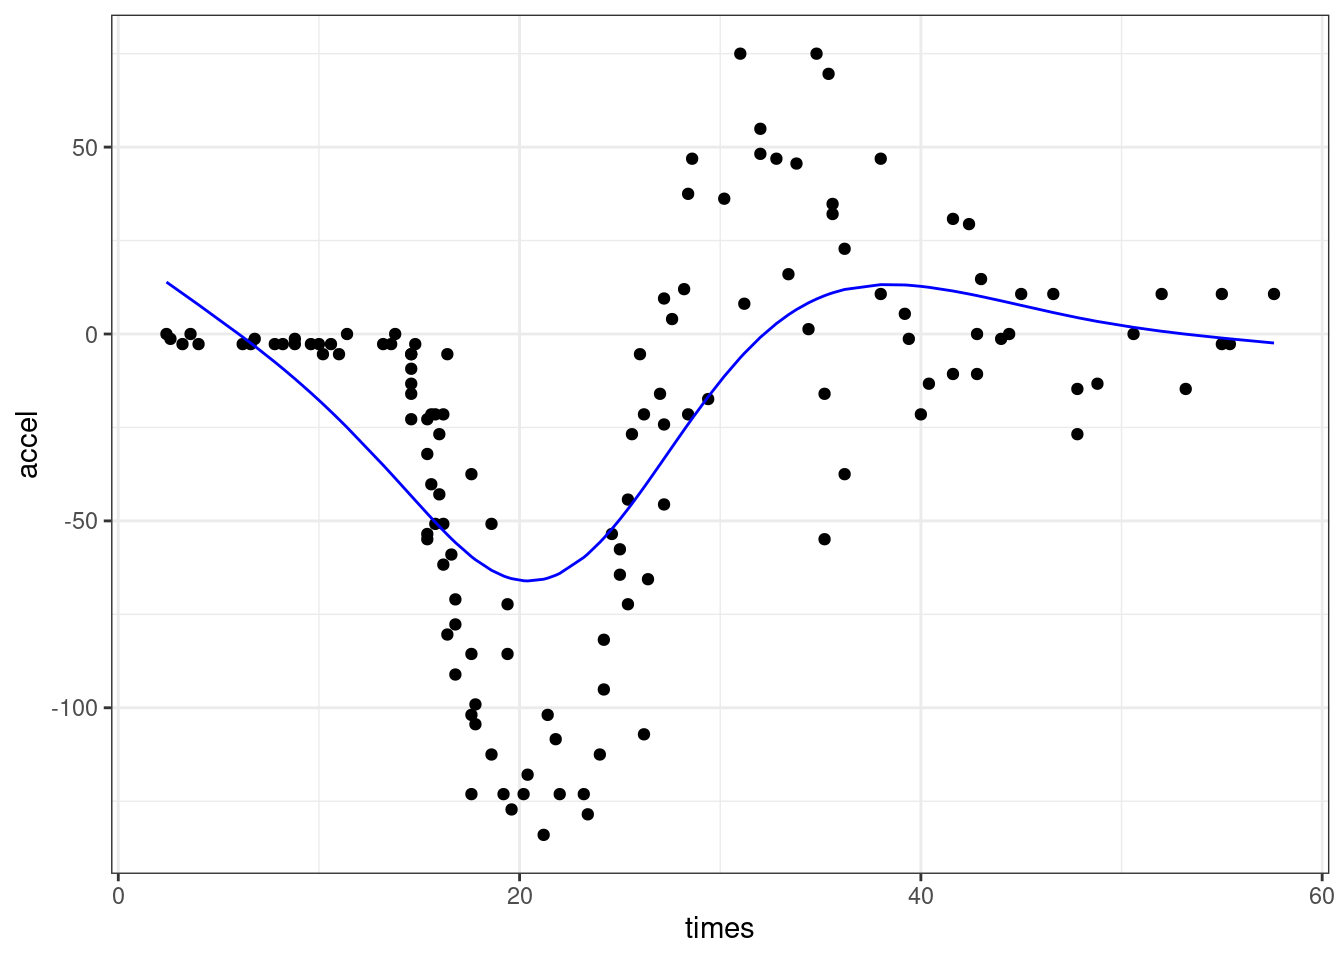
\includegraphics{1.-Regresja-liniowa_files/figure-latex/unnamed-chunk-1-1.pdf}

Załóżmy, że istnieje zalezność pomiędzy wiekiem, a wzrostem. Mówiąc
dokładniej załózmy, że istnieje pewna \textbf{nieznana deterministyczna
(nielosowa)} funckcja \texttt{f} taka, że:

\texttt{wzrost\ =\ f(wiek)\ +\ epsilon}.

W ogólnym przypadku gdy mamy \texttt{N} zmiennych
\texttt{(X\_1,\ X\_2,\ ...,\ X\_N)} zwanych \textbf{predyktorami}
(zmiennymi objaśniającymi) oraz \textbf{zmienną objaśnianą} \texttt{Y}
relację tę zapiszemy jako

\texttt{Y\ =\ f(X\_1,\ X\_2,\ ...,\ X\_N)\ +\ epsilon}.

W tym miejscu należy zadać 2 pytania. Po pierwsze czym jest
\texttt{epsilon} i po drugie, czy nie może on zostać wykluczony z
naszego równania?

\texttt{epsilon} okreslany jest często zwyczajnie mianem \textbf{błędu
losowego}, jednakże warto zastanowić się skąd bierze się ten błąd?
Wyobraźmy sobie, że udzielamy kredytu na podstawie pewnych predyktorów
będących danymi o kliencie: zarobki, wydatki, stan cywilny, liczba
dzieci itd. itp. Czy majac 2 klientów banku starających się o kredyt,
posiadających identyczne wartości tych zmiennych jesteśmy pewni, że ich
spłata (bądź brak spłaty) kredytu bedzie identyczny? Odpowiedź brzmi
nie, poza informacjami zgromadzownymi przez bank istnieje jeszcze wiele
różnych innych zmiennych (np. to czy dana osoba jest hazardzistą,
wypadki itp.), które mogą wpłynąć na wynik. Z tego też powodu o
\texttt{epsilon} warto myśleć jako o \textbf{niewiedzy o pewnych
zjawiskach, które nie zostały ujęte w naszych danych} zamiast jako o
sztucznym błędzie losowym.

Wróćmy jednak do naszego zadania. Założyliśmy pewną relację pomiędzy
wielkiem dziecka a jego wzrostem. Czy jesteśmy w stanie odnaleźć tę
relację, czyli znaleźć funkcję \texttt{f}? Nie do końca, \texttt{f} może
być dowolną funkcją. W tym miejscu zamiast szukać dowolnej funkcji,
dodamy kilka dodatkowych założeń na jej temat tworząc pewien
\textbf{model statystyczny}. W praktyce oznacza to, ze zamiast szukać
funckji \texttt{f} szukać będziemy funkcji \texttt{f\textquotesingle{}}
zakładając, że:

\texttt{wzrost\ \textasciitilde{}\ f\textquotesingle{}(wiek)}

Model statystyczny oznacza pewne \textbf{uproszczenie rzeczywistości}, w
którym funkcja \texttt{f\textquotesingle{}} reprezentuje \texttt{f} w
pewien \textbf{``optymalny''} sposób. Wrócimy jeszcze do tego co oznacza
optymalna reprezentacja.

Jednym z najprostszych modeli statystycznych jest model \textbf{regresji
liniowej}, w którym zakładamy, że \texttt{f\textquotesingle{}} jest
funkcją liniową naszych predyktorów. W naszym przypadku:

\texttt{wzrost\ \textasciitilde{}\ beta\_0\ +\ beta\_1*wiek},

gdzie \texttt{beta\_0} i \texttt{beta\_1} sa pewnymi stałymi, które
będziemy chcieli \textbf{wyestymować}.

Zwizualizyjmy założenia naszego modelu dla kliku przykładowych
\texttt{beta\_0} i \texttt{beta\_1}:

\begin{Shaded}
\begin{Highlighting}[]
\NormalTok{beta\_}\DecValTok{0}\NormalTok{\_list \textless{}{-}}\StringTok{ }\KeywordTok{c}\NormalTok{(}\DecValTok{60}\NormalTok{, }\DecValTok{65}\NormalTok{, }\DecValTok{79}\NormalTok{)}
\NormalTok{beta\_}\DecValTok{1}\NormalTok{\_list \textless{}{-}}\StringTok{ }\KeywordTok{c}\NormalTok{(}\FloatTok{0.9}\NormalTok{, }\FloatTok{0.6}\NormalTok{, }\FloatTok{{-}0.3}\NormalTok{)}
\NormalTok{test\_lines \textless{}{-}}\StringTok{ }\KeywordTok{map2\_df}\NormalTok{(beta\_}\DecValTok{0}\NormalTok{\_list, beta\_}\DecValTok{1}\NormalTok{\_list, }\OperatorTok{\textasciitilde{}}\StringTok{ }\NormalTok{\{}
\NormalTok{  beta\_}\DecValTok{0}\NormalTok{ \textless{}{-}}\StringTok{ }\NormalTok{.x}
\NormalTok{  beta\_}\DecValTok{1}\NormalTok{ \textless{}{-}}\StringTok{ }\NormalTok{.y}
\NormalTok{  beta \textless{}{-}}\StringTok{ }\KeywordTok{paste}\NormalTok{(}\StringTok{"beta\_0:"}\NormalTok{, beta\_}\DecValTok{0}\NormalTok{, }\StringTok{"beta\_1:"}\NormalTok{, beta\_}\DecValTok{1}\NormalTok{, }\DataTypeTok{collapse =} \StringTok{" "}\NormalTok{)}
  \KeywordTok{tibble}\NormalTok{(}
    \DataTypeTok{age =} \KeywordTok{seq}\NormalTok{(}\DecValTok{18}\NormalTok{, }\DecValTok{29}\NormalTok{, }\DataTypeTok{by =} \FloatTok{0.1}\NormalTok{),}
    \DataTypeTok{height =}\NormalTok{ beta\_}\DecValTok{0} \OperatorTok{+}\StringTok{ }\NormalTok{beta\_}\DecValTok{1} \OperatorTok{*}\StringTok{ }\NormalTok{age,}
    \DataTypeTok{beta =}\NormalTok{ beta}
\NormalTok{  )}
\NormalTok{\})}
\KeywordTok{ggplot}\NormalTok{(age\_height, }\KeywordTok{aes}\NormalTok{(age, height)) }\OperatorTok{+}\StringTok{ }\KeywordTok{theme\_bw}\NormalTok{() }\OperatorTok{+}\StringTok{ }\KeywordTok{geom\_point}\NormalTok{() }\OperatorTok{+}
\StringTok{  }\KeywordTok{geom\_line}\NormalTok{(}\DataTypeTok{data =}\NormalTok{ test\_lines, }\KeywordTok{aes}\NormalTok{(}\DataTypeTok{color =}\NormalTok{ beta))}
\end{Highlighting}
\end{Shaded}

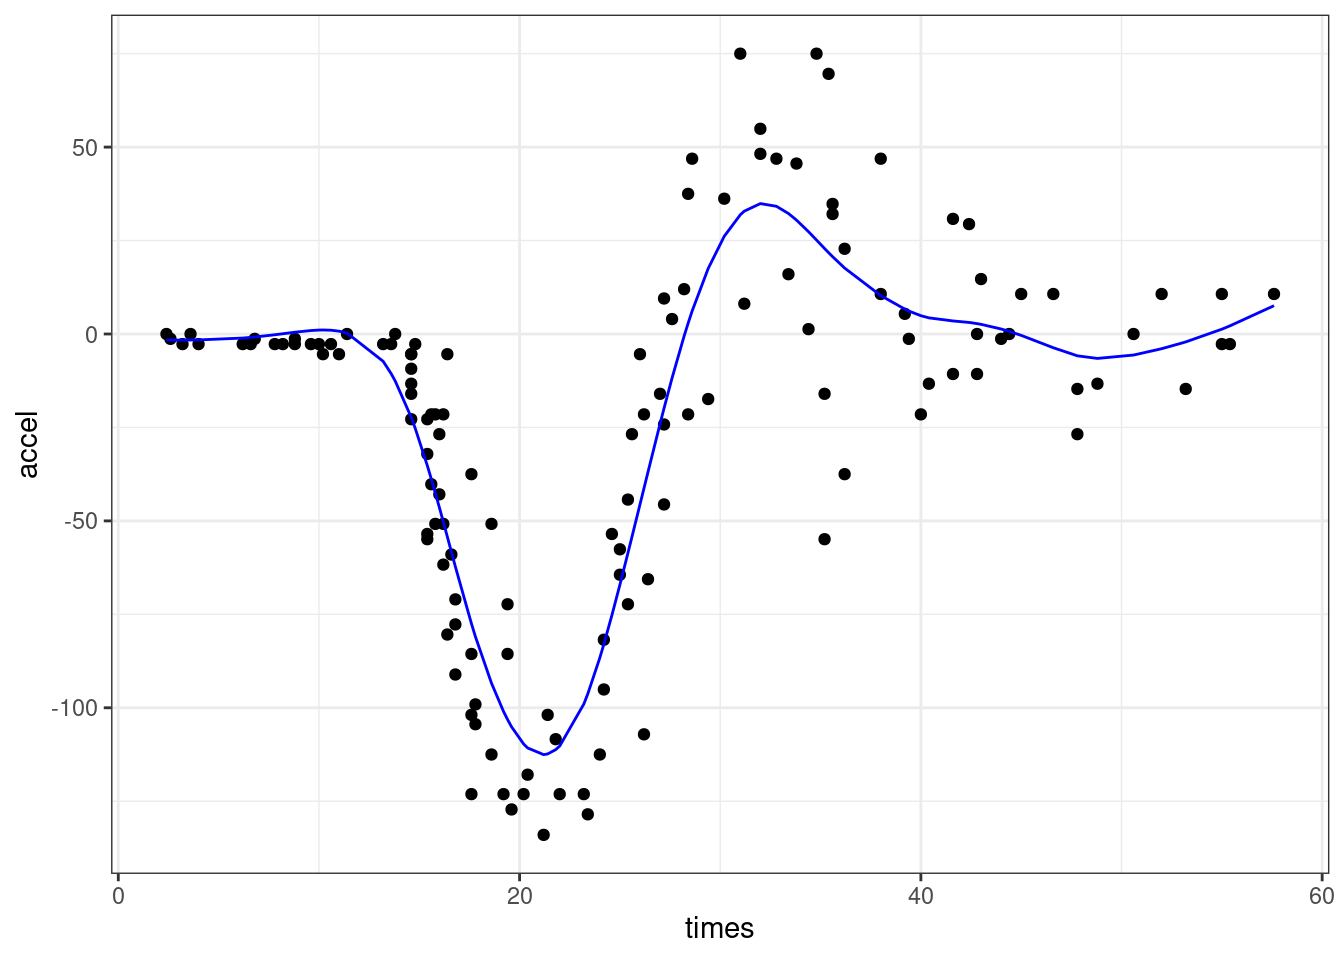
\includegraphics{1.-Regresja-liniowa_files/figure-latex/unnamed-chunk-2-1.pdf}

Oczywiście nasuwa nam się pytanie jak wybrac parametry \texttt{beta\_0}
i \texttt{beta\_1} aby nasze rozwiązanie było \textbf{optymalne}. Aby je
wybrać musimy sobie najpierw odpowiedzieć na pytanie co oznacza
optymalność naszego rozwiązania? Oczywistym jest to iż chcemy, aby nasze
\textbf{predykcje} były jak najlepsze - najbliższe prawdziwym wartościom
wieku. Potrzebna jest nam jednak metoda mierzenia optymalności.

W ogólnym przypadku po wybraniu modelu statystycznego wybieramy tak
zwaną \textbf{funkcję straty}, której wartości bedziemy chcieli
\textbf{mimimalizować}. W przypadku regresji liniowej standardowym
wyborem jest \textbf{błąd sredniokwadratowy} - średnia kwadratów różnić
pomiędzy prawdziwymi wartościami (wzrostu), a predykcjami z modelu.
Szukamy więc \texttt{beta\_0} i \texttt{beta\_1}, które zminimalizują
błąd sredniokwadratowy. Jest to tak zwana \textbf{Metoda najmnieszych
kwadratów}.

\texttt{MSE(beta\_0,\ beta\_1)\ =\ średnia((wzrost\ -\ (beta\_0\ +\ beta\_1*wiek))\^{}2)}

Policzmy więc błąd średniokwadratowy dla 3 wartości z poprzedniego
przykładu:

\begin{Shaded}
\begin{Highlighting}[]
\NormalTok{beta\_}\DecValTok{0}\NormalTok{\_list \textless{}{-}}\StringTok{ }\KeywordTok{c}\NormalTok{(}\DecValTok{60}\NormalTok{, }\DecValTok{65}\NormalTok{, }\DecValTok{79}\NormalTok{)}
\NormalTok{beta\_}\DecValTok{1}\NormalTok{\_list \textless{}{-}}\StringTok{ }\KeywordTok{c}\NormalTok{(}\FloatTok{0.9}\NormalTok{, }\FloatTok{0.6}\NormalTok{, }\FloatTok{{-}0.3}\NormalTok{)}
\KeywordTok{map2\_df}\NormalTok{(beta\_}\DecValTok{0}\NormalTok{\_list, beta\_}\DecValTok{1}\NormalTok{\_list, }\OperatorTok{\textasciitilde{}}\StringTok{ }\NormalTok{\{}
\NormalTok{  beta\_}\DecValTok{0}\NormalTok{ \textless{}{-}}\StringTok{ }\NormalTok{.x}
\NormalTok{  beta\_}\DecValTok{1}\NormalTok{ \textless{}{-}}\StringTok{ }\NormalTok{.y}
\NormalTok{  beta \textless{}{-}}\StringTok{ }\KeywordTok{paste}\NormalTok{(}\StringTok{"beta\_0:"}\NormalTok{, beta\_}\DecValTok{0}\NormalTok{, }\StringTok{"beta\_1:"}\NormalTok{, beta\_}\DecValTok{1}\NormalTok{, }\DataTypeTok{collapse =} \StringTok{" "}\NormalTok{)}
\NormalTok{  age\_height }\OperatorTok{\%\textgreater{}\%}
\StringTok{    }\KeywordTok{mutate}\NormalTok{(}\DataTypeTok{prediction\_height =}\NormalTok{ beta\_}\DecValTok{0} \OperatorTok{+}\StringTok{ }\NormalTok{beta\_}\DecValTok{1} \OperatorTok{*}\StringTok{ }\NormalTok{age,}
           \DataTypeTok{beta =}\NormalTok{ beta)}
\NormalTok{\}) }\OperatorTok{\%\textgreater{}\%}
\StringTok{  }\KeywordTok{group\_by}\NormalTok{(beta) }\OperatorTok{\%\textgreater{}\%}
\StringTok{  }\KeywordTok{summarise}\NormalTok{(}\DataTypeTok{MSE =} \KeywordTok{mean}\NormalTok{((height }\OperatorTok{{-}}\StringTok{ }\NormalTok{prediction\_height)}\OperatorTok{\^{}}\DecValTok{2}\NormalTok{))}
\end{Highlighting}
\end{Shaded}

\begin{verbatim}
## # A tibble: 3 x 2
##   beta                       MSE
##   <chr>                    <dbl>
## 1 beta_0: 60 beta_1: 0.9   2.58 
## 2 beta_0: 65 beta_1: 0.6   0.632
## 3 beta_0: 79 beta_1: -0.3 72.9
\end{verbatim}

Jak widać najmniejszy błąd dostaliśmy dla wartości
\texttt{beta\_0:\ 65\ beta\_1:\ 0.6}. Jak jednak dobrać \texttt{beta\_0}
i \texttt{beta\_1} aby błąd był najmniejszy? Matematyczne rozwiązanie
tego problemu dane jest wzorem:

\begin{Shaded}
\begin{Highlighting}[]
\NormalTok{X \textless{}{-}}\StringTok{ }\KeywordTok{cbind}\NormalTok{(}\DecValTok{1}\NormalTok{, age\_height}\OperatorTok{$}\NormalTok{age)}
\NormalTok{y \textless{}{-}}\StringTok{ }\NormalTok{age\_height}\OperatorTok{$}\NormalTok{height}
\KeywordTok{solve}\NormalTok{(}\KeywordTok{t}\NormalTok{(X)}\OperatorTok{\%*\%}\NormalTok{X)}\OperatorTok{\%*\%}\KeywordTok{t}\NormalTok{(X)}\OperatorTok{\%*\%}\NormalTok{y}
\end{Highlighting}
\end{Shaded}

\begin{verbatim}
##           [,1]
## [1,] 64.928322
## [2,]  0.634965
\end{verbatim}

w R współczynniki regresji liniowe możemy policzyc z użyciem funkcji
\texttt{lm}:

\begin{Shaded}
\begin{Highlighting}[]
\NormalTok{lin\_reg \textless{}{-}}\StringTok{ }\KeywordTok{lm}\NormalTok{(height }\OperatorTok{\textasciitilde{}}\StringTok{ }\NormalTok{age, age\_height)}
\NormalTok{lin\_reg}
\end{Highlighting}
\end{Shaded}

\begin{verbatim}
## 
## Call:
## lm(formula = height ~ age, data = age_height)
## 
## Coefficients:
## (Intercept)          age  
##      64.928        0.635
\end{verbatim}

Zwizualizujmy wyniki:

\begin{Shaded}
\begin{Highlighting}[]
\NormalTok{beta\_}\DecValTok{0}\NormalTok{ \textless{}{-}}\StringTok{ }\FloatTok{64.928322}
\NormalTok{beta\_}\DecValTok{1}\NormalTok{ \textless{}{-}}\StringTok{ }\FloatTok{0.634965}
\NormalTok{beta \textless{}{-}}\StringTok{ }\KeywordTok{paste}\NormalTok{(}\StringTok{"beta\_0:"}\NormalTok{, }\KeywordTok{round}\NormalTok{(beta\_}\DecValTok{0}\NormalTok{, }\DecValTok{2}\NormalTok{), }\StringTok{"beta\_1:"}\NormalTok{, }\KeywordTok{round}\NormalTok{(beta\_}\DecValTok{1}\NormalTok{, }\DecValTok{2}\NormalTok{), }\DataTypeTok{collapse =} \StringTok{" "}\NormalTok{)}
\NormalTok{best\_line \textless{}{-}}\StringTok{  }\KeywordTok{tibble}\NormalTok{(}
  \DataTypeTok{age =} \KeywordTok{seq}\NormalTok{(}\DecValTok{18}\NormalTok{, }\DecValTok{29}\NormalTok{, }\DataTypeTok{by =} \FloatTok{0.1}\NormalTok{),}
  \DataTypeTok{height =}\NormalTok{ beta\_}\DecValTok{0} \OperatorTok{+}\StringTok{ }\NormalTok{beta\_}\DecValTok{1} \OperatorTok{*}\StringTok{ }\NormalTok{age,}
  \DataTypeTok{beta =}\NormalTok{ beta}
\NormalTok{)}
\KeywordTok{ggplot}\NormalTok{(age\_height, }\KeywordTok{aes}\NormalTok{(age, height)) }\OperatorTok{+}\StringTok{ }\KeywordTok{theme\_bw}\NormalTok{() }\OperatorTok{+}\StringTok{ }\KeywordTok{geom\_point}\NormalTok{() }\OperatorTok{+}
\StringTok{  }\KeywordTok{geom\_line}\NormalTok{(}\DataTypeTok{data =}\NormalTok{ best\_line, }\KeywordTok{aes}\NormalTok{(}\DataTypeTok{color =}\NormalTok{ beta))}
\end{Highlighting}
\end{Shaded}

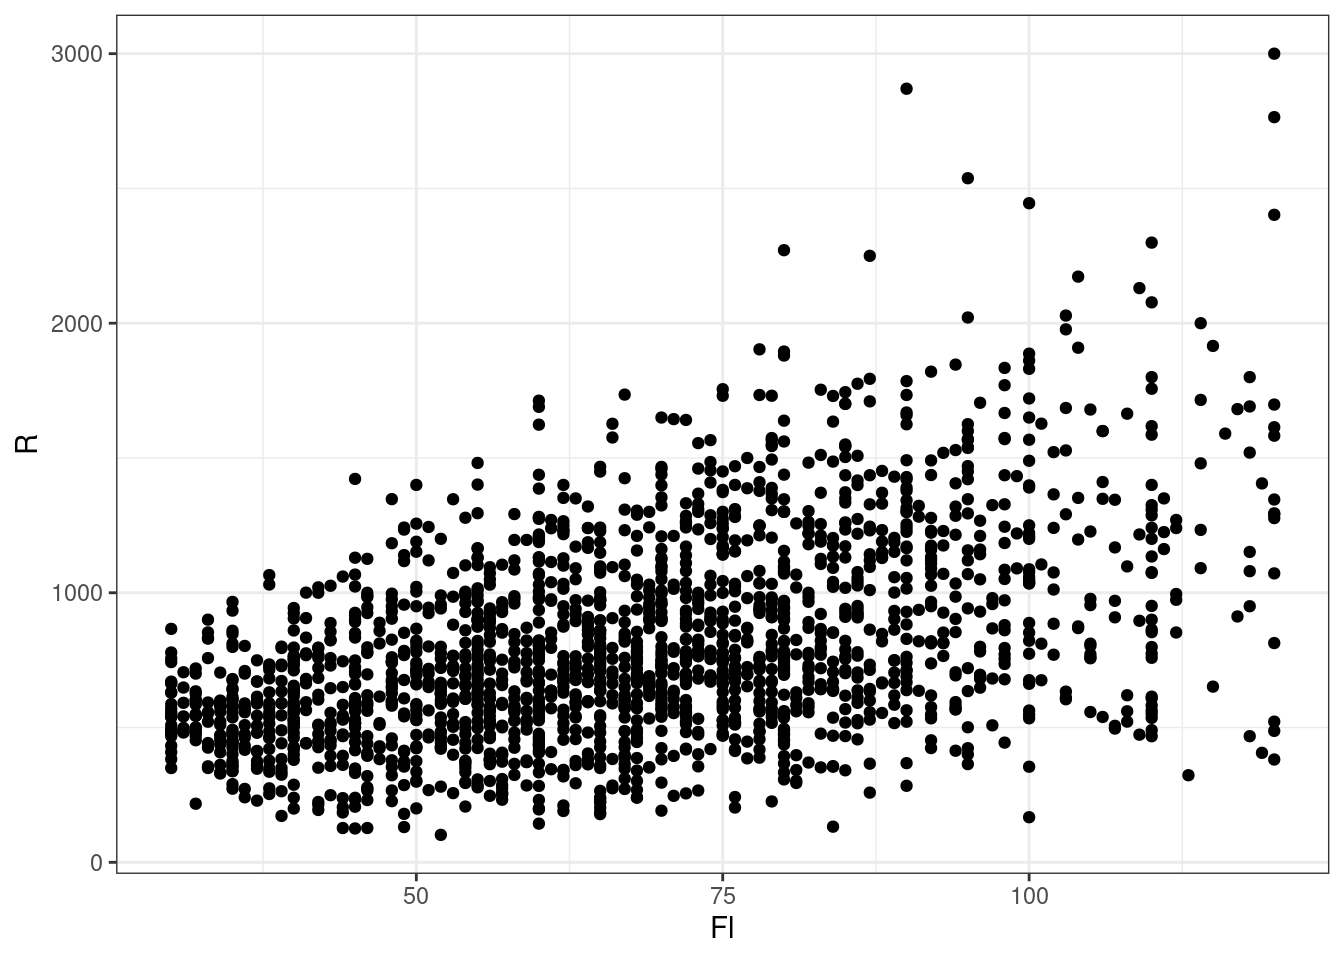
\includegraphics{1.-Regresja-liniowa_files/figure-latex/unnamed-chunk-6-1.pdf}

I sprawdźmy ile wynosi błąd średniokwadratowy:

\begin{Shaded}
\begin{Highlighting}[]
\KeywordTok{mean}\NormalTok{(lin\_reg}\OperatorTok{$}\NormalTok{residuals}\OperatorTok{\^{}}\DecValTok{2}\NormalTok{)}
\end{Highlighting}
\end{Shaded}

\begin{verbatim}
## [1] 0.0545979
\end{verbatim}

Wartosci \texttt{beta\_0} i \texttt{beta\_1}, które tutaj otrzymaliśmy
są optymalne dla błędu średniokwadratowego, można by się zastanowić co
by było gdybyśmy wybrali inną funkcję straty np. \textbf{błąd absolutny}
- średnia różnic wartości bezwzględnych pomiędzy prawdziwymi wartościami
(wzrostu), a predykcjami z modelu. Błąd absolutny jest lepszym wybrem
gdy mamy do czynienia z wartościami odstającymi, ale o tym
później\ldots{}

\newpage

\hypertarget{metoda-najwiux119kszej-wiarygodnoux15bci}{%
\subsection{Metoda największej
wiarygodności}\label{metoda-najwiux119kszej-wiarygodnoux15bci}}

Metoda najmniejszych kwadratów jest bardzo prosta do zrozumienia,
jednkże jej minusem jest to, że nie nie ma ona głębszych założeń np o
rozkładach, przez co nie jesteśmy w stanie powiedziec o naszym modelu
nic więcej. Jedną z rzeczy, które mogłbyby nas interesować to czy
wyliczone współczynniki \texttt{beta\_0} i \texttt{beta\_1} są
statystycznie istotone (są niezerowe) lub czy cały model jest (czy
faktycznie istnieje liniowa zależność).

przejdziemy teraz do \textbf{metody największej wiarygodności}, która
towarzyszyć nam będzie w trakcie poznawania kolejnych modeli. Zanim
zastosujemy ją do regresji liniowej, zacznijmy od prosszego modelu, w
którym chcemy ustalić jakie jest prawdopodobieństwo wyrzucenia orła przy
rzucie monetą (być może fałszywą).

Zacznijmy od wygenerowania przykładowych rzutów:

\begin{Shaded}
\begin{Highlighting}[]
\KeywordTok{set.seed}\NormalTok{(}\DecValTok{1234}\NormalTok{)}
\NormalTok{coins \textless{}{-}}\StringTok{ }\KeywordTok{rbinom}\NormalTok{(}\DecValTok{20}\NormalTok{, }\DecValTok{1}\NormalTok{, }\FloatTok{0.3}\NormalTok{)}
\NormalTok{coins}
\end{Highlighting}
\end{Shaded}

\begin{verbatim}
##  [1] 0 0 0 0 1 0 0 0 0 0 0 0 0 1 0 1 0 0 0 0
\end{verbatim}

Metoda największej wiarygodności działa następująco:

\begin{enumerate}
\def\labelenumi{\arabic{enumi}.}
\tightlist
\item
  Na samym początku musimy znaleźć \textbf{funkcje wiarygodności}. Aby
  tego dokonać musimy znać rozkład z jakiego pochodzą nasze dane (albo
  go założyć!). W naszym przypadku dane do wyniki rzutu monetą, gdzie
  możemy otrzymać tylko orła lub reszkę. Jest to więć
  \href{https://pl.wikipedia.org/wiki/Rozk\%C5\%82ad_zero-jedynkowy}{rozkład
  Bernulliego}. Prawdopodobienstwo wyrzucenia orła wynosi \texttt{p}, a
  reszki \texttt{1\ -\ p}. Funkcja wiarygodności dla obserwacji będzie
  równa:
\end{enumerate}

\texttt{p\^{}x\ *\ (1\ -\ p)\^{}(1\ -\ x)} gdzie \texttt{x} to rezultat
rzutu tzn. \texttt{x\ =\ 0} lub \texttt{x\ =\ 1}

Kolejnym krokiem jest utworzenie funkcji wiarygodności dla całości -
produkt wiarygodności poszczególnych obserwacji:

\texttt{p\^{}k\ *\ (1\ -\ p)\^{}(N\ -\ k)} gdzie \texttt{k} to liczba
orłów, a \texttt{N} to liczba rzutów. W naszym konkretnym przypadku:

\texttt{p\^{}3\ *\ (1\ -\ p)\^{}(20\ -\ 3)}

\begin{enumerate}
\def\labelenumi{\arabic{enumi}.}
\setcounter{enumi}{1}
\tightlist
\item
  Maksymalizujemy funkcje wiarygodności ze względu na szukany parametr
  \texttt{p}
\end{enumerate}

\begin{Shaded}
\begin{Highlighting}[]
\NormalTok{likelihood\_coins \textless{}{-}}\StringTok{ }\KeywordTok{tibble}\NormalTok{(}
  \DataTypeTok{p =} \KeywordTok{seq}\NormalTok{(}\DecValTok{0}\NormalTok{, }\DecValTok{1}\NormalTok{, }\DataTypeTok{by =} \FloatTok{0.001}\NormalTok{),}
  \DataTypeTok{likelihood =}\NormalTok{ p}\OperatorTok{\^{}}\DecValTok{3} \OperatorTok{*}\StringTok{ }\NormalTok{(}\DecValTok{1} \OperatorTok{{-}}\StringTok{ }\NormalTok{p)}\OperatorTok{\^{}}\NormalTok{(}\DecValTok{20} \DecValTok{{-}3}\NormalTok{)}
\NormalTok{)}
\KeywordTok{ggplot}\NormalTok{(likelihood\_coins, }\KeywordTok{aes}\NormalTok{(p, likelihood)) }\OperatorTok{+}\StringTok{ }\KeywordTok{theme\_bw}\NormalTok{() }\OperatorTok{+}\StringTok{ }\KeywordTok{geom\_line}\NormalTok{()}
\end{Highlighting}
\end{Shaded}

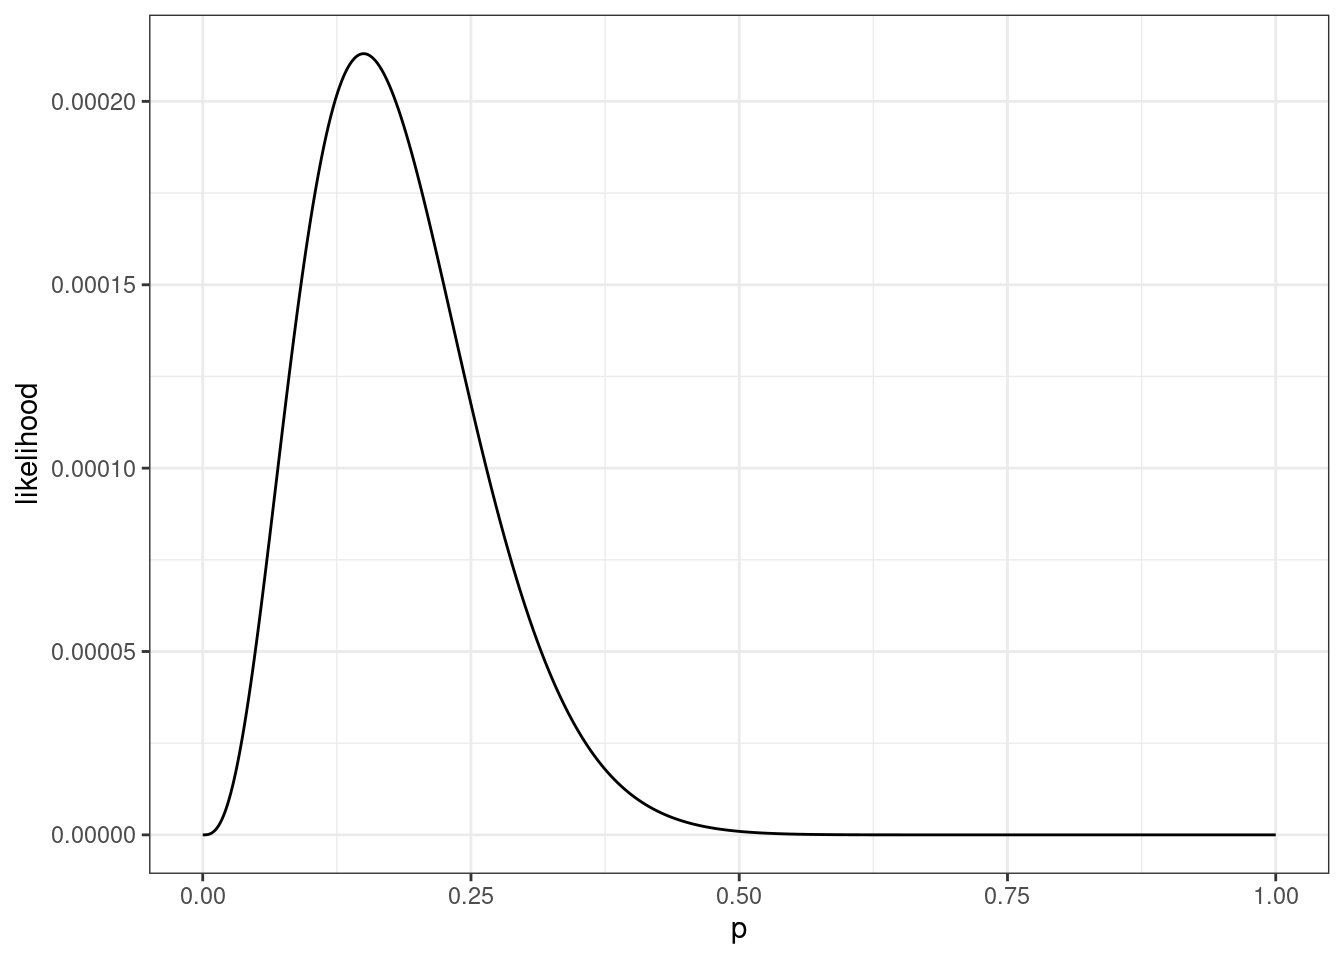
\includegraphics{1.-Regresja-liniowa_files/figure-latex/unnamed-chunk-9-1.pdf}

Łatwo zauważyć, że maksimum otrzymujemy dla \texttt{p\ =\ 0.15}

\begin{Shaded}
\begin{Highlighting}[]
\NormalTok{likelihood\_coins }\OperatorTok{\%\textgreater{}\%}\StringTok{ }\KeywordTok{filter}\NormalTok{(likelihood }\OperatorTok{==}\StringTok{ }\KeywordTok{max}\NormalTok{(likelihood))}
\end{Highlighting}
\end{Shaded}

\begin{verbatim}
## # A tibble: 1 x 2
##       p likelihood
##   <dbl>      <dbl>
## 1  0.15   0.000213
\end{verbatim}

No dobrze, ale jak to się ma do regresji liniowej (i pokrewnych modeli)?

W modelu regresji liniowej zakładamy, że \textbf{warunkowa wartość
oczekiwana} (uogólniając średnia) \texttt{y\textbar{}X} (wzrost pod
warunkiem wieku) pochodzi z rozkładu normalnego o sredniej zaleznej
liniowo od predyktorów (wieku w naszym przypadku):

\texttt{y\textbar{}X\ \textasciitilde{}\ N(u,\ sigma),\ u\ =\ X*beta}

gdzie zakładamy stałą wartość \texttt{sigma} (odchylenie standardowe)

\newpage

Jak dokładnie rozumieć tę zależność? Myślmy o tym w ten sposób: Jeśli
mam ustaloną wartość wieku dziecka np. 18 miesięcy to wzrost dzieci w
wieku 18 miesięcy pochodzi z rozkładu normalnego o sredniej
\texttt{beta\_0\ +\ beta\_1\ *\ 18} (\texttt{beta\_0} i \texttt{beta\_1}
estymujemy metodą największej wiarygodności).

\begin{figure}
\centering
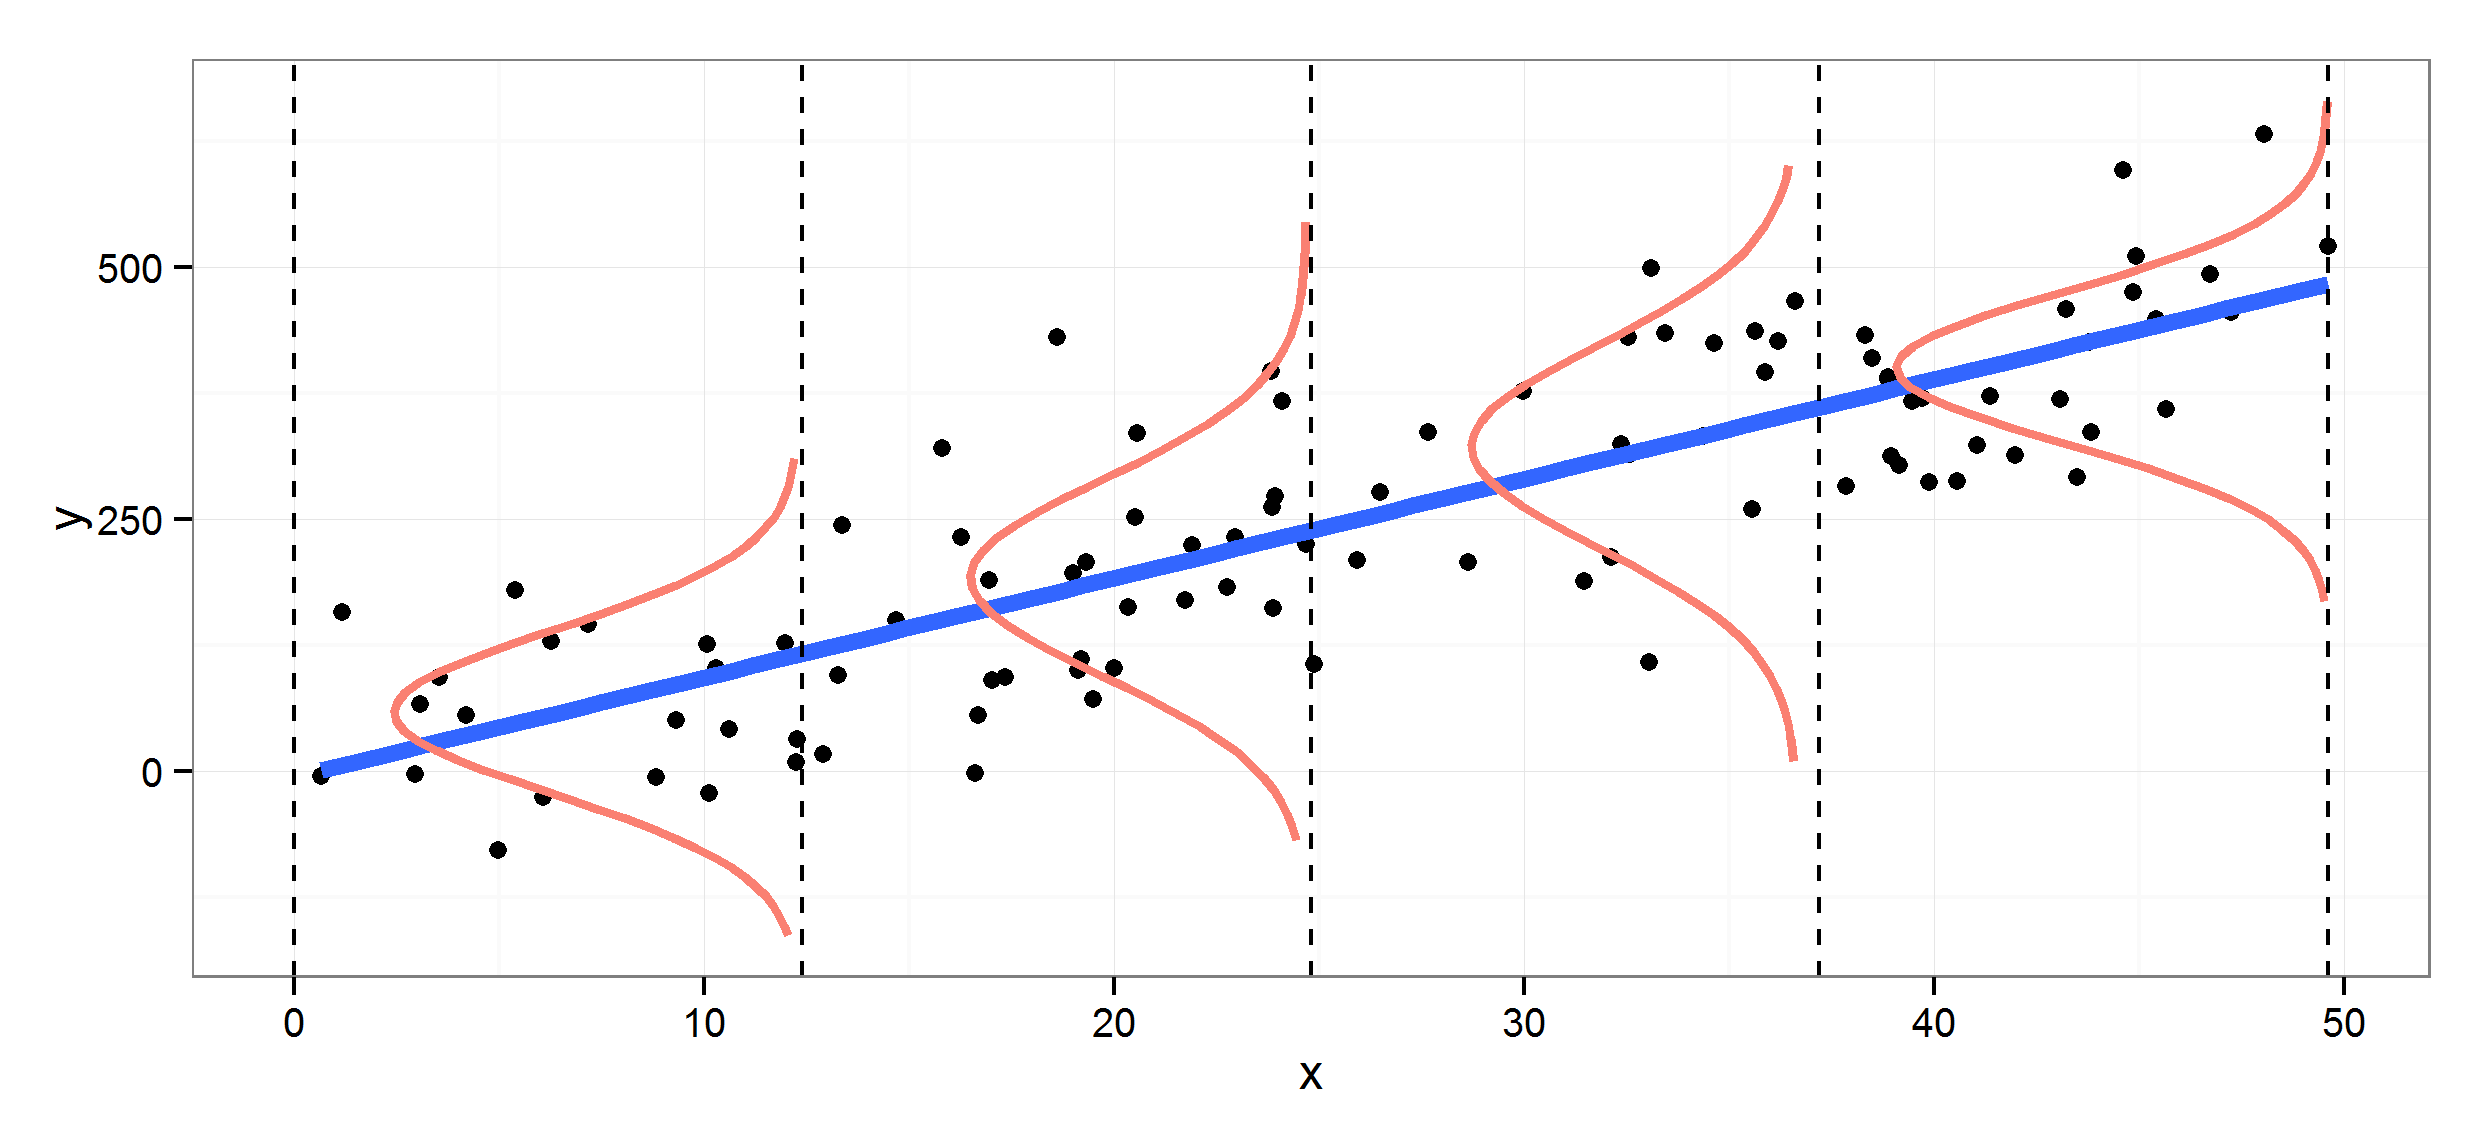
\includegraphics{"imgs/reg_lin.png"}
\caption{Założenia regresji liniowej}
\end{figure}

Nie wchodząc za głęboko w teorię matematyczną, funkcja największej
wiarygodności dla regresji liniowej dana jest wzorem:

\begin{figure}
\centering
\includegraphics{"imgs/reg_lin_likelihood.png"}
\caption{Likelihood regresji liniowej}
\end{figure}

Bardzo często zamiast maksymalizować funkcję wiarygodności mozemy
maksymalizować jej logarytm (log-likelihood) ponieważ jest to prostsza
funkcja (z własności logarytmu wiemy że maksymalizacja obu jest
równowazna.)

\begin{figure}
\centering
\includegraphics{"imgs/reg_lin_likelihood2.png"}
\caption{Log-Likelihood regresji liniowej}
\end{figure}

Okazuje się, że w przypadku regresji liniowej log-likelihood jest
``przesuniętym'' błędem sredniokwadratowym co oznacza, że minimalizacja
błądu średniokwadratowego jest równoważna maksymalizacji log-likelihood
- z obu metod mamy ten sam wynik.

\includegraphics{"imgs/reg_lin_likelihood3.png"}

\begin{figure}
\centering
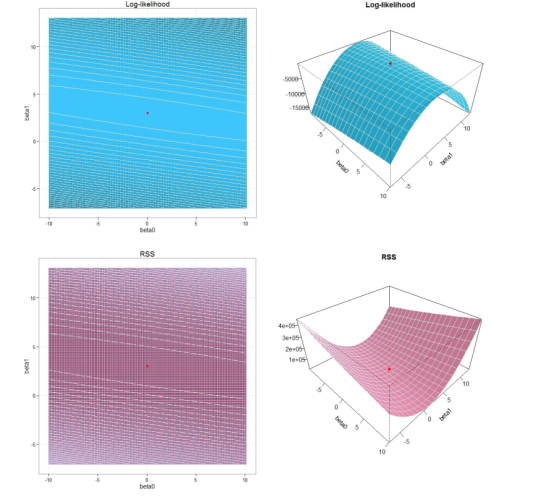
\includegraphics{"imgs/reg_lin_likelihood4.png"}
\caption{Log-Likelihood regresji liniowej jako MSE}
\end{figure}

Ten sam wynik, jednakże mamy teraz założenia o rozkładzie, co daje nam
duże możliwości:

\begin{Shaded}
\begin{Highlighting}[]
\KeywordTok{summary}\NormalTok{(lin\_reg)}
\end{Highlighting}
\end{Shaded}

\begin{verbatim}
## 
## Call:
## lm(formula = height ~ age, data = age_height)
## 
## Residuals:
##      Min       1Q   Median       3Q      Max 
## -0.27238 -0.24248 -0.02762  0.16014  0.47238 
## 
## Coefficients:
##             Estimate Std. Error t value Pr(>|t|)    
## (Intercept)  64.9283     0.5084  127.71  < 2e-16 ***
## age           0.6350     0.0214   29.66 4.43e-11 ***
## ---
## Signif. codes:  0 '***' 0.001 '**' 0.01 '*' 0.05 '.' 0.1 ' ' 1
## 
## Residual standard error: 0.256 on 10 degrees of freedom
## Multiple R-squared:  0.9888, Adjusted R-squared:  0.9876 
## F-statistic:   880 on 1 and 10 DF,  p-value: 4.428e-11
\end{verbatim}

Jak interpretowac wyniki tego podsumowania:

\begin{enumerate}
\def\labelenumi{\arabic{enumi}.}
\tightlist
\item
  Współczynniki (Coefficients):
\end{enumerate}

\begin{itemize}
\item
  \texttt{beta\_0} (Intercept) - Jeśli wszystkie predyktory mają wartość
  \texttt{0} to wartość zmiennej objasnianej bedzie równa
  \texttt{beta\_0}. Jednakże wartość ta nie powinna być zawsze
  tłumaczona (uzasadniana) ponieważ w wielu przypadkach nie ma to sensu.
  W naszym przykładzie (jesli się uprzeć i tłumaczyć) byłby to średni
  wzrost dziecka mierzony od razu po narodzinach.
\item
  \texttt{beta\_1/2/.../N} - Mówią o ile wzrośnie/zmaleje wartośc
  zmiennej objasnianej jeśli wartość predyktora wzrośnie/zmaleje. w
  naszym przykładzie jesli dziecko zestarzeje się o \texttt{1} miesiąc
  to jego wzrost bedzie wiekszy o \texttt{1\ *\ 0.6350} cm.
\item
  przy każdym współczynniku widnieje wartość statystyki \texttt{t} oraz
  \textbf{p-value}. Nie wchodząć w szczegóły statystyczne dzięki
  założenim normalności regresji liniowej znamy rozkład współczynników i
  możemy użyc t-testu by sprawdzić czy wartość współczynnika jest
  niezerowa (to znaczy zmienna jest istotna).
\end{itemize}

Zobaczmy co się stanie gdy dodamy losową zmienną do naszego modelu:

\begin{Shaded}
\begin{Highlighting}[]
\NormalTok{age\_height\_plus\_random  \textless{}{-}}\StringTok{ }\NormalTok{age\_height }\OperatorTok{\%\textgreater{}\%}
\StringTok{  }\KeywordTok{mutate}\NormalTok{(}\DataTypeTok{random =} \KeywordTok{runif}\NormalTok{(}\KeywordTok{nrow}\NormalTok{(age\_height)))}
\KeywordTok{summary}\NormalTok{(}\KeywordTok{lm}\NormalTok{(height }\OperatorTok{\textasciitilde{}}\StringTok{ }\NormalTok{age }\OperatorTok{+}\StringTok{ }\NormalTok{random, age\_height\_plus\_random))}
\end{Highlighting}
\end{Shaded}

\begin{verbatim}
## 
## Call:
## lm(formula = height ~ age + random, data = age_height_plus_random)
## 
## Residuals:
##      Min       1Q   Median       3Q      Max 
## -0.28157 -0.23100 -0.00811  0.13586  0.49335 
## 
## Coefficients:
##             Estimate Std. Error t value Pr(>|t|)    
## (Intercept)  64.9363     0.5307 122.355 8.26e-16 ***
## age           0.6326     0.0230  27.503 5.39e-10 ***
## random        0.1182     0.2725   0.434    0.675    
## ---
## Signif. codes:  0 '***' 0.001 '**' 0.01 '*' 0.05 '.' 0.1 ' ' 1
## 
## Residual standard error: 0.267 on 9 degrees of freedom
## Multiple R-squared:  0.989,  Adjusted R-squared:  0.9865 
## F-statistic: 404.4 on 2 and 9 DF,  p-value: 1.539e-09
\end{verbatim}

\begin{enumerate}
\def\labelenumi{\arabic{enumi}.}
\setcounter{enumi}{1}
\tightlist
\item
  F-statistic:
\end{enumerate}

\begin{itemize}
\tightlist
\item
  Ten test bada czy model jako całość jest istotny, a dokładniej czy
  dopasowanie naszego modelu jest statystycznie lepsze od dopasowania
  modelu bez predyktorów (dopasowanie zwykłą srednią ze zmiennej
  objaśnianej). Hipotera zerowa mówi, że nie jest. Możemy myślec o tym
  tescie jako o teście odpowiedniego doboru modelu (jeśli nasz model nie
  jest lepszy od zwykłej sredniej to może założenia o liniowości nie są
  poprawne w tym przypadku).
\end{itemize}

\begin{enumerate}
\def\labelenumi{\arabic{enumi}.}
\setcounter{enumi}{2}
\tightlist
\item
  Multiple R-squared i Adjusted R-squared:
\end{enumerate}

\begin{itemize}
\tightlist
\item
  Obie są metrykami dopasowania modelu. Wachają się od 0 do 1. im blizej
  1 tym lepsze dopasowanie modelu. Mierzą procent wariancji danych
  wyjaśnianą przez model. Adjusted R-squared bierze poprawkę na ilość
  predyktorów w modelu. Duże różnice między tymi współczynnikami moga
  wskazywać na przedopasowanie (overfitting) modelu.
\end{itemize}

\begin{Shaded}
\begin{Highlighting}[]
\NormalTok{age\_height\_plus\_multiple\_random  \textless{}{-}}\StringTok{ }\NormalTok{age\_height }\OperatorTok{\%\textgreater{}\%}
\StringTok{  }\KeywordTok{select}\NormalTok{(}\OperatorTok{{-}}\NormalTok{age)}
\ControlFlowTok{for}\NormalTok{ (i }\ControlFlowTok{in} \DecValTok{1}\OperatorTok{:}\DecValTok{10}\NormalTok{) \{}
\NormalTok{  age\_height\_plus\_multiple\_random \textless{}{-}}\StringTok{ }\NormalTok{age\_height\_plus\_multiple\_random }\OperatorTok{\%\textgreater{}\%}
\StringTok{  }\KeywordTok{mutate}\NormalTok{(}\OperatorTok{!!}\KeywordTok{sym}\NormalTok{(}\KeywordTok{paste0}\NormalTok{(}\StringTok{"random"}\NormalTok{, i)) }\OperatorTok{:}\ErrorTok{=}\StringTok{ }\KeywordTok{runif}\NormalTok{(}\KeywordTok{nrow}\NormalTok{(age\_height)))}
\NormalTok{\}}
\KeywordTok{summary}\NormalTok{(}\KeywordTok{lm}\NormalTok{(height }\OperatorTok{\textasciitilde{}}\StringTok{ }\NormalTok{., age\_height\_plus\_multiple\_random))}
\end{Highlighting}
\end{Shaded}

\begin{verbatim}
## 
## Call:
## lm(formula = height ~ ., data = age_height_plus_multiple_random)
## 
## Residuals:
##        1        2        3        4        5        6        7        8 
## -1.53678 -0.93805 -0.50369  0.12267  0.57984  1.37003  0.79833 -1.05726 
##        9       10       11       12 
## -0.01895  0.97580  0.70093 -0.49286 
## 
## Coefficients:
##             Estimate Std. Error t value Pr(>|t|)  
## (Intercept)   77.314     12.006   6.439   0.0981 .
## random1      -10.837     18.806  -0.576   0.6672  
## random2       -4.997      8.062  -0.620   0.6468  
## random3       -4.246      4.448  -0.954   0.5148  
## random4        3.548      4.963   0.715   0.6049  
## random5        4.168      4.490   0.928   0.5236  
## random6       14.572     15.721   0.927   0.5241  
## random7        7.805      5.191   1.504   0.3736  
## random8       -3.004      4.811  -0.624   0.6447  
## random9        3.014     10.936   0.276   0.8288  
## random10       3.323     10.493   0.317   0.8047  
## ---
## Signif. codes:  0 '***' 0.001 '**' 0.01 '*' 0.05 '.' 0.1 ' ' 1
## 
## Residual standard error: 3.027 on 1 degrees of freedom
## Multiple R-squared:  0.8428, Adjusted R-squared:  -0.729 
## F-statistic: 0.5362 on 10 and 1 DF,  p-value: 0.798
\end{verbatim}

\end{document}
